%%%%%%%%%%%%%%%%%%%%%%%%%%%%%%%%%%%%%%%%%
% Structured General Purpose Assignment
% LaTeX Template
%
% This template has been downloaded from:
% http://www.latextemplates.com
%
% Original author:
% Ted Pavlic (http://www.tedpavlic.com)
%
% Note:
% The \lipsum[#] commands throughout this template generate dummy text
% to fill the template out. These commands should all be removed when
% writing assignment content.
%
%%%%%%%%%%%%%%%%%%%%%%%%%%%%%%%%%%%%%%%%%

%----------------------------------------------------------------------------------
%   PACKAGES AND OTHER DOCUMENT CONFIGURATIONS
%----------------------------------------------------------------------------------

\documentclass{article}

\usepackage[utf8]{inputenc}
\usepackage[spanish]{babel}
\usepackage{fancyhdr} % Required for custom headers
\usepackage{lastpage} % Required to determine the last page for the footer
\usepackage{graphicx} % Required to insert images
\usepackage{enumitem}
\usepackage{environ}
\usepackage{multicol}
\usepackage{hyperref}
\usepackage[font=small]{caption}
\usepackage{pifont}
\selectlanguage{spanish}
\addto\extrasspanish{%
    \def\figureautorefname{Figura}%
}
\newcommand{\myarrow}{\ding{223}}
\newcommand{\cmark}{\ding{51}}
\newcommand{\xmark}{\ding{55}}

% Margins
\topmargin=-0.45in
\evensidemargin=0in
\oddsidemargin=0in
\textwidth=6.5in
\textheight=9.0in
\headsep=0.25in

\linespread{1.1} % Line spacing

% Set up the header and footer
\pagestyle{fancy}
\lhead{\small \hmwkClass: \hmwkTitle} % Top left header
\chead{} % Top center header
\rhead{\small \hmwkAuthorName} % Top right header
\lfoot{} % Bottom left footer
\cfoot{} % Bottom center footer
\rfoot{Página\ \thepage\ de\ \pageref{LastPage}} % Bottom right footer
\renewcommand\headrulewidth{0.4pt} % Size of the header rule
\renewcommand\footrulewidth{0.4pt} % Size of the footer rule

\setlength\parindent{0pt} % Removes all indentation from paragraphs
\setlength{\multicolsep}{6.0pt plus 2.0pt minus 1.5pt} % 50% of original values

\newlength\widest
\makeatletter
\NewEnviron{ldescription}{%
    \vbox{%
        \global\setlength\widest{0pt}%
        \def\item[##1]{%
            \settowidth\@tempdima{\textbf{##1}}%
            \ifdim \@tempdima>\widest \global\setlength\widest{\@tempdima} \fi%
        }%
        \setbox0=\hbox{\BODY}%
    }
    \begin{description}[leftmargin=\dimexpr\widest+0.5em\relax,labelindent=16pt, labelwidth=\widest]
        \BODY
\end{description}%
}
\makeatother

%----------------------------------------------------------------------------------
%   NAME AND CLASS SECTION
%----------------------------------------------------------------------------------

\newcommand{\hmwkTitle}{Práctica\ 2} % Assignment title
\newcommand{\hmwkClass}{Sistemas Informáticos I} % Course/class
\newcommand{\hmwkClassTime}{10:30am} % Class/lecture time
\newcommand{\hmwkAuthorName}{\small Sergio Fuentes de Uña | Daniel Perdices Burrero} % Your name

%----------------------------------------------------------------------------------
%   TITLE PAGE
%----------------------------------------------------------------------------------

\title{
    \vspace{2in}
    \textmd{\textbf{\hmwkClass:\ \hmwkTitle}}\\
    \normalsize\vspace{0.1in}\small{\today}\\
    \vspace{3in}
}

\author{\textbf{\hmwkAuthorName}}
\date{} % Insert date here if you want it to appear below your name

%----------------------------------------------------------------------------------

\begin{document}

\maketitle

%----------------------------------------------------------------------------------
%   TABLE OF CONTENTS
%----------------------------------------------------------------------------------

%\setcounter{tocdepth}{1} % Uncomment this line if you don't want subsections listed in the ToC

\newpage
\tableofcontents
\newpage

\section{Archivos}
La entrega final de la práctica está compuesta por los siguientes archivos:
\begin{ldescription}
    \item[$\bullet$ \texttt{index.php}]
        Página principal del sitio web ({\small\autoref{fig:fig1}}).
    \item[$\bullet$ \texttt{matches.php}]
        Listado de partidos disponibles para apostar ({\small\autoref{fig:fig1}, \autoref{fig:fig2}, \autoref{fig:fig3}}).
    \item[$\bullet$ \texttt{register.php}]
        Formulario de registro de un nuevo usuario.
    \item[$\bullet$ \texttt{bet.php}]
        Formulario de realización de una apuesta.
    \item[$\bullet$ \texttt{checkout.php}]
        Administración del carrito de apuestas.
    \item[$\bullet$ \texttt{credit.php}]
        Administración de saldo del usuario.
    \item[$\bullet$ \texttt{history.php}]
        Historial de apuestas del usuario.
    \item[$\bullet$ \texttt{usercount.php}]
        Banner con número de usuarios conectados.
    \item[$\bullet$ \texttt{theme.css}]
        Hoja de estilo CSS del sitio web.
    \item[$\bullet$ \texttt{functions.js}]
        Librería de funciones JavaScript.
    \item[$\bullet$ \texttt{db.xml}]
        Conjunto de apuestas disponibles en XML.
    \item[$\bullet$ \texttt{users/}]
        Directorio de datos de los usuarios.
    \item[$\bullet$ \texttt{games/}]
        Directorio de recursos gráficos para las apuestas.
    \item[$\bullet$ \texttt{images/}]
        Directorio de recursos gráficos de propósito general.
    \item[$\bullet$ \texttt{Memoria-P2.pdf}]
        Memoria del trabajo realizado (este archivo).
\end{ldescription}
\newpage
\section{Instrucciones de uso}
\subsection{Encontrar una apuesta}
Al acceder a la página principal se muestra el conjunto de todas las apuestas, organizadas en dos secciones:
\begin{itemize}
    \item\textbf{\textit{Upcoming Matches}}: Encuentros que aún no se han celebrado o que aún no han terminado y por los que se puede apostar, los más inminentes aparecen primero.
        \smallskip\newline
        \begin{minipage}{\linewidth}
            \centering
            \captionsetup{type=figure}
            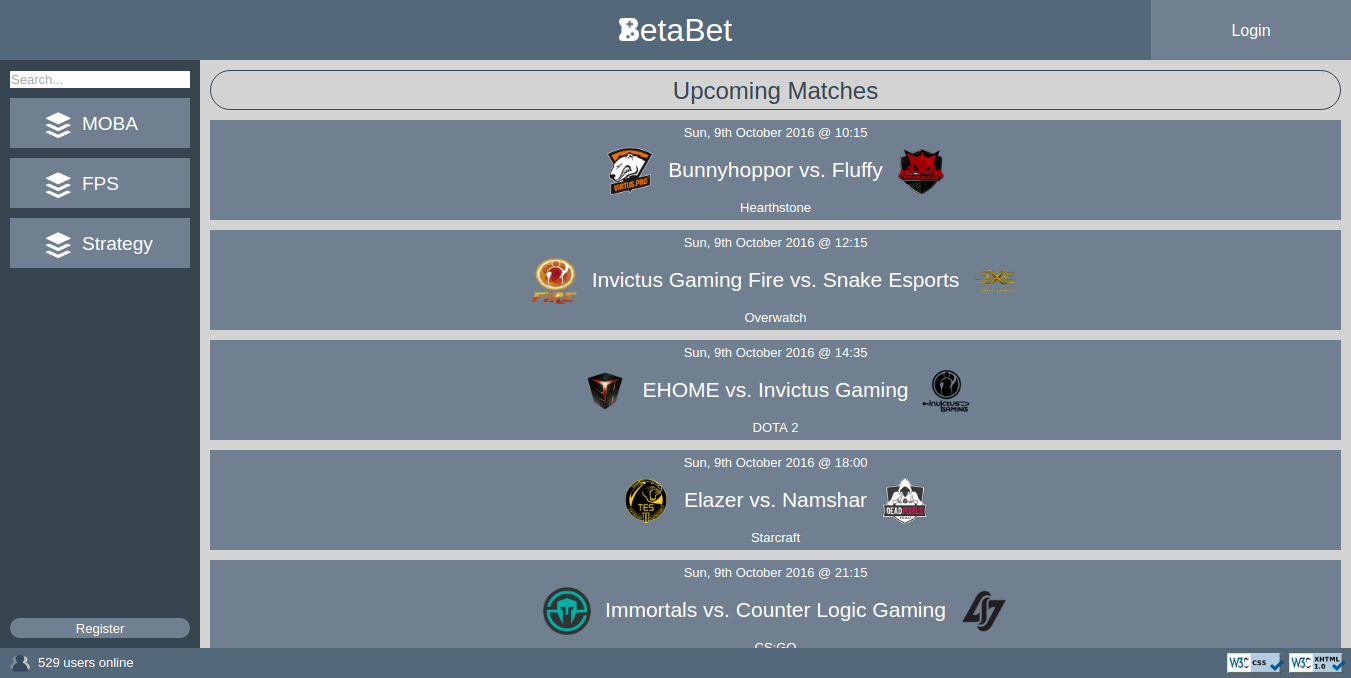
\includegraphics[width=\linewidth]{fig1}
            \caption{\textit{Upcoming Matches}}
            \label{fig:fig1}
        \end{minipage}
    \item\textbf{\textit{Latest Matches}}: Encuentros finalizados por los que ya no es posible apostar y cuyos resultados se indican en la página, los más recientes aparecen primero.\
        \smallskip\newline
        \begin{minipage}{\linewidth}
            \centering
            \captionsetup{type=figure}
            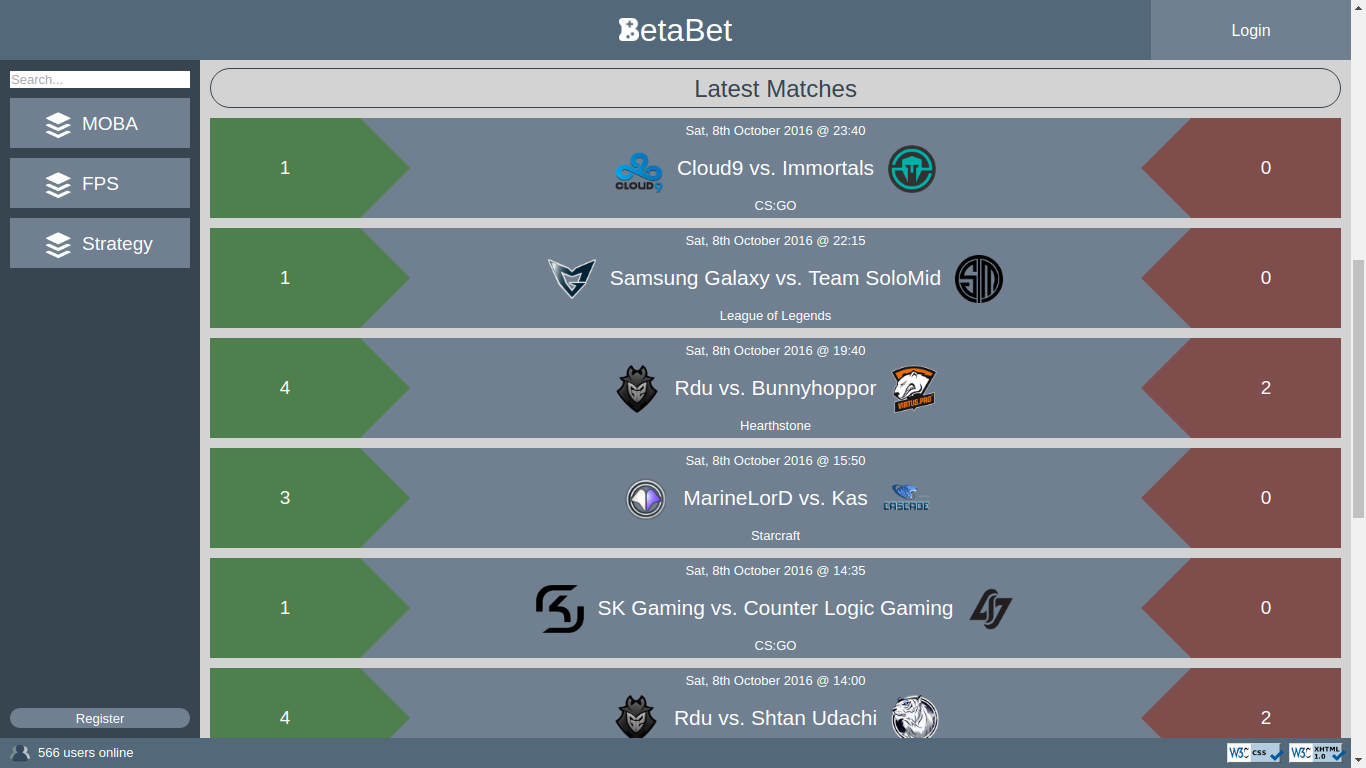
\includegraphics[width=\linewidth]{fig2}
            \caption{\textit{Latest Matches}}
            \label{fig:fig2}
        \end{minipage}
\end{itemize}
\newpage
Existen dos mecanismos de filtrado de apuestas para localizar encuentros según unos intereses determinados:
\begin{itemize}
    \item\textbf{Categorías}: Desplegando los menús del panel lateral y pulsando los botones correspondientes es posible mostrar únicamente las apuestas de una cierta categoría.
        \smallskip\newline
        \begin{minipage}{\linewidth}
            \centering
            \captionsetup{type=figure}
            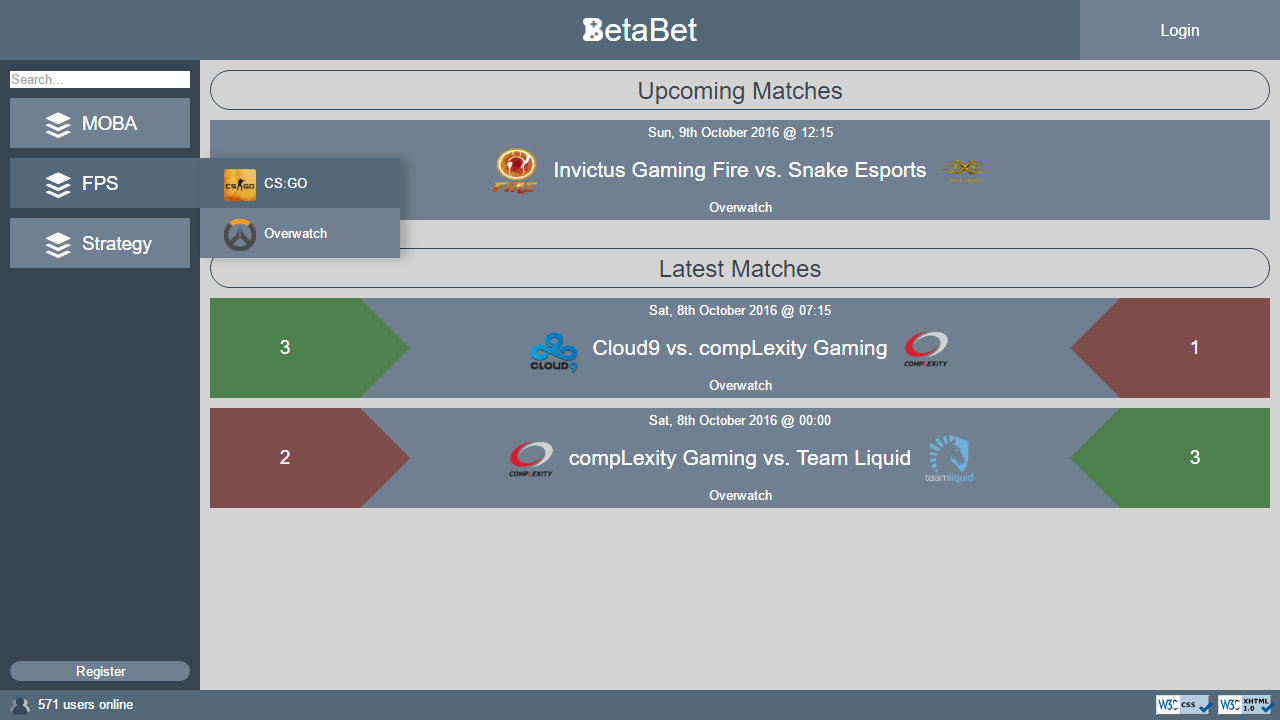
\includegraphics[width=\linewidth]{fig3}
            \caption{Filtrado por categorías}
            \label{fig:fig3}
        \end{minipage}
    \item\textbf{Búsqueda}: Escribiendo directamente en el campo de búsqueda del panel lateral se filtran automáticamente las apuestas cuyos datos coinciden con el patrón buscado.
        \smallskip\newline
        \begin{minipage}{\linewidth}
            \centering
            \captionsetup{type=figure}
            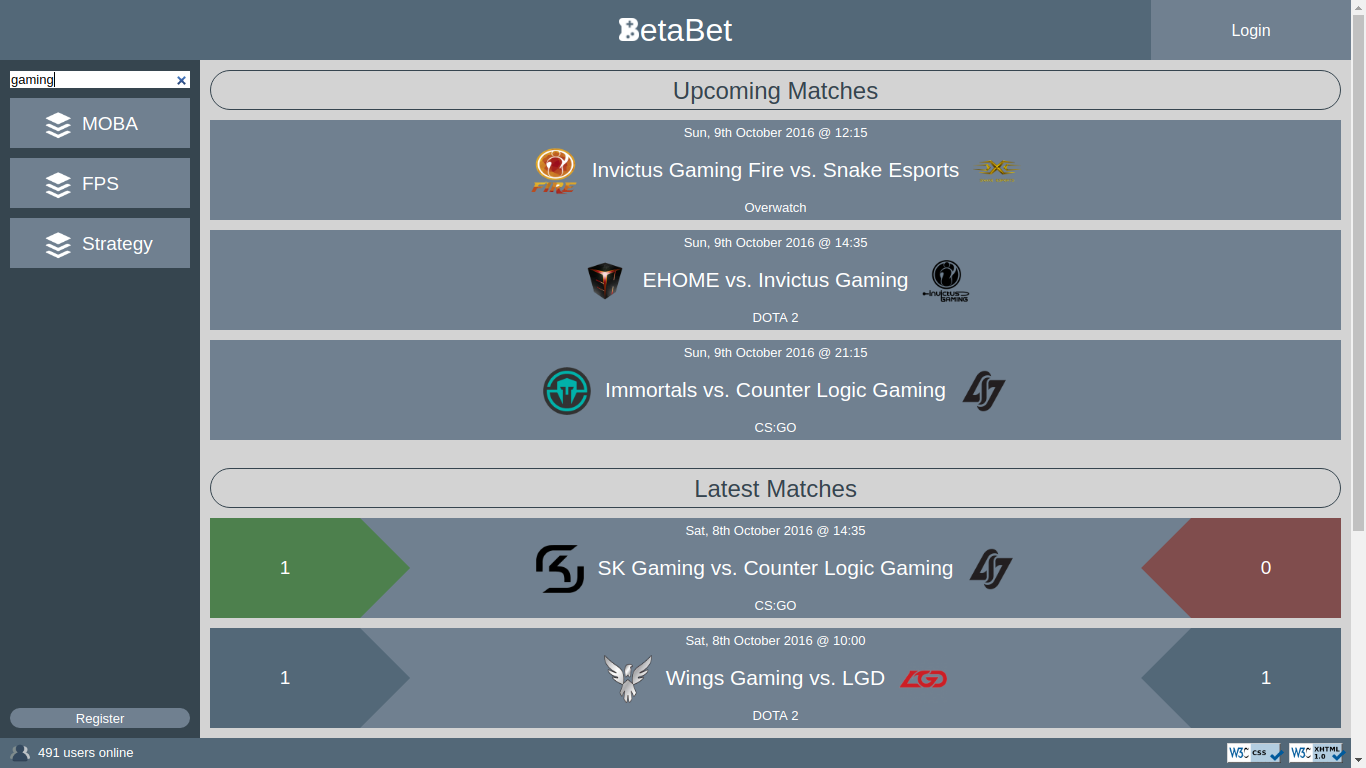
\includegraphics[width=\linewidth]{fig4}
            \caption{Filtrado por búsqueda}
            \label{fig:fig4}
        \end{minipage}
\end{itemize}
\newpage
\subsection{Realizar una apuesta}
Una vez localizada la apuesta deseada, basta con hacer clic en ella para acceder al formulario de apuesta.
\smallskip\newline
\begin{minipage}{\linewidth}
    \centering
    \captionsetup{type=figure}
    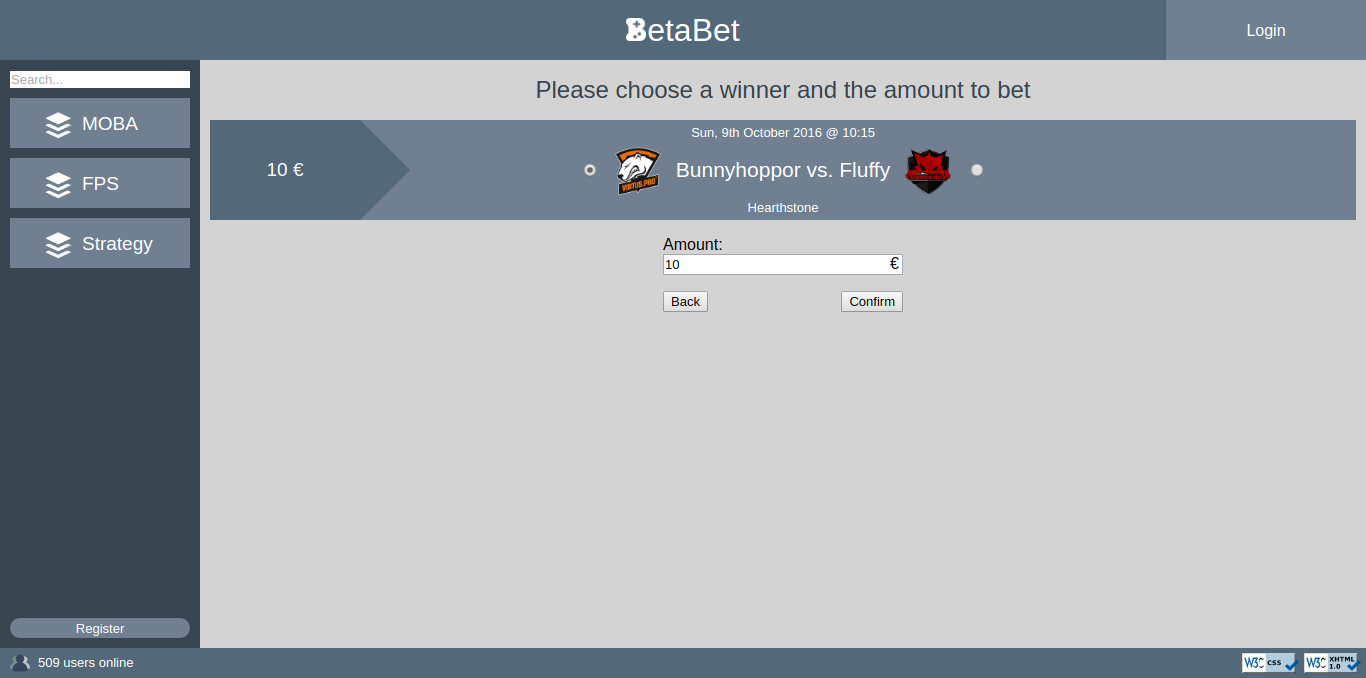
\includegraphics[width=\linewidth]{fig5}
    \caption{Formulario de apuesta}
    \label{fig:fig5}
\end{minipage}
\smallskip\newline
Tras confirmar un ganador y una cantidad para apostar, se comprueba la validez de los datos introducidos.
\begin{multicols}{4}
    \begin{center}
        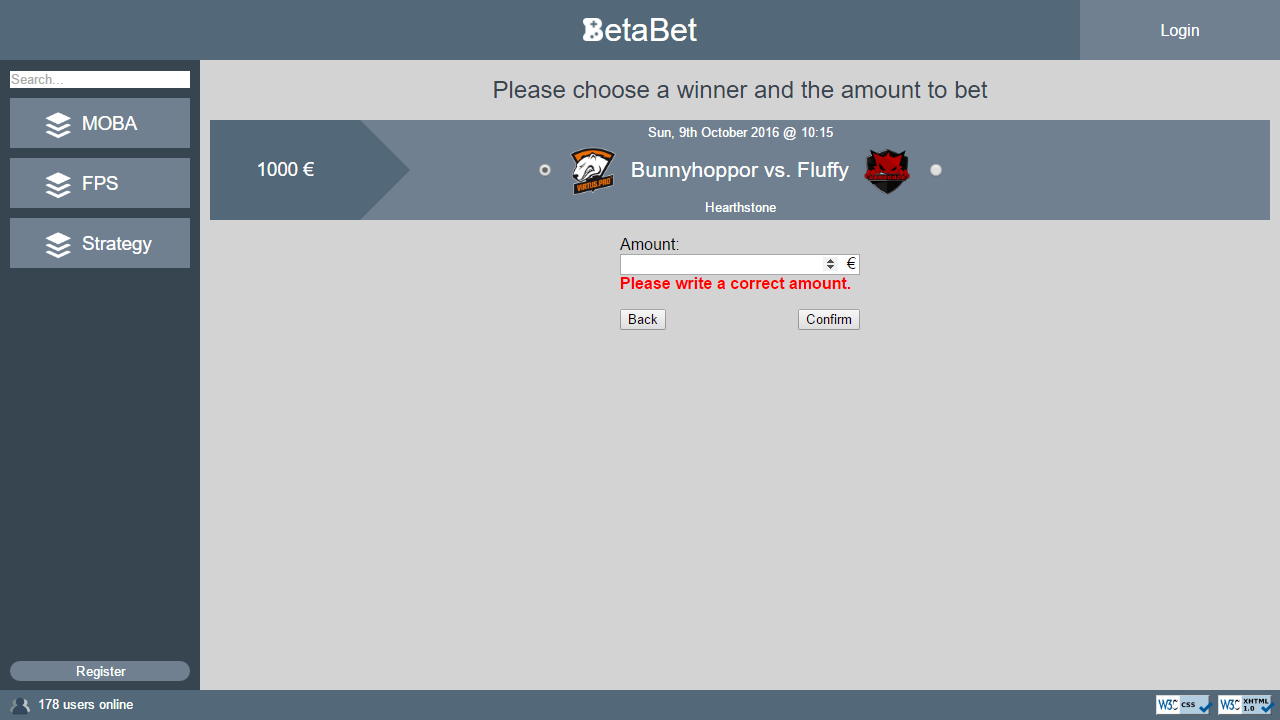
\includegraphics[width=.975\linewidth]{bet1}
        Formato incorrecto
    \end{center}
    \columnbreak
    \begin{center}
        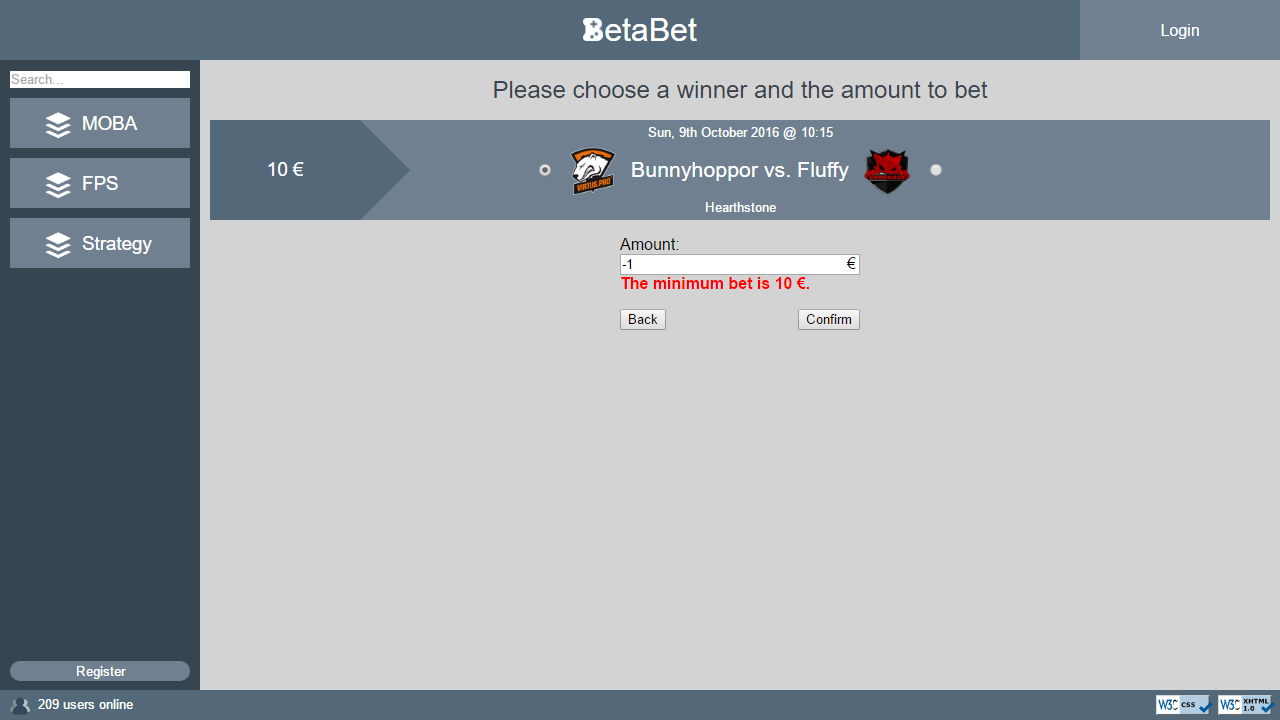
\includegraphics[width=.975\linewidth]{bet2}
        Apuesta muy pequeña
    \end{center}
    \columnbreak
    \begin{center}
        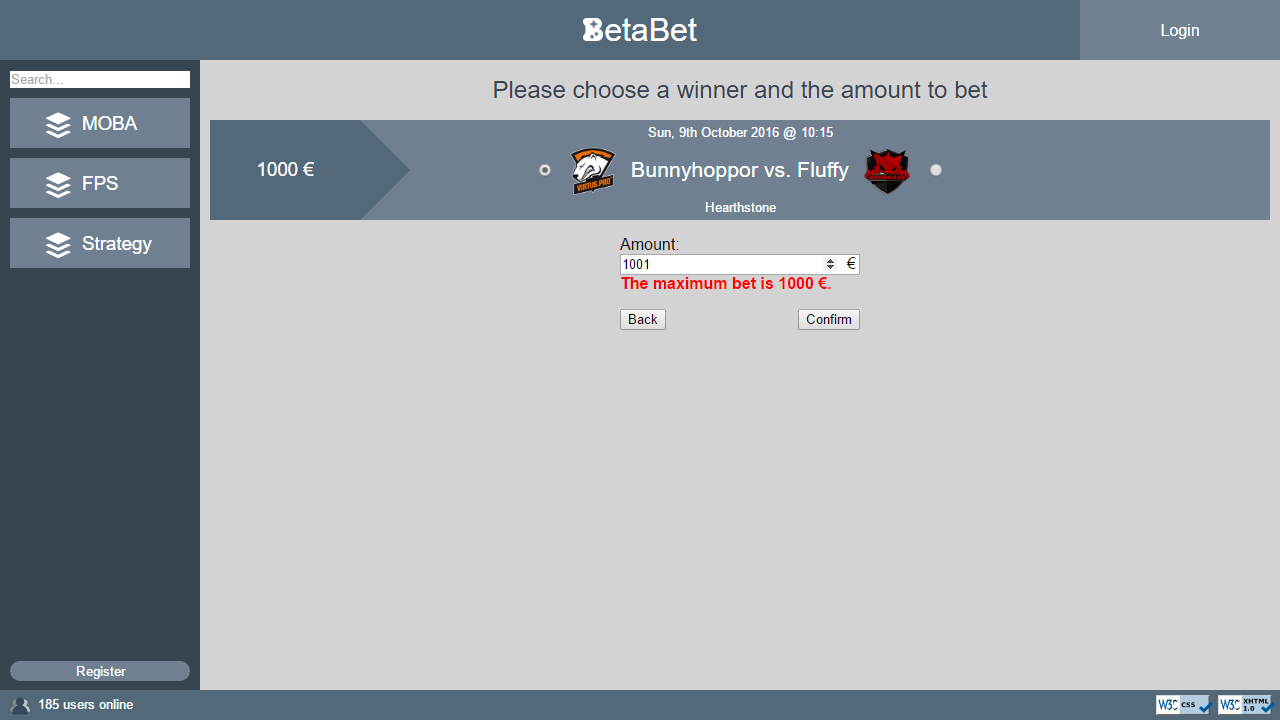
\includegraphics[width=.975\linewidth]{bet3}
        Apuesta muy grande
    \end{center}
    \columnbreak
    \begin{center}
        
\includegraphics[width=.975\linewidth]{bet4}
        Céntimos no permitidos
    \end{center}
\end{multicols}
Cuando se confirma una apuesta válida, se muestra una confirmación y posteriormente se añade al carrito.
\smallskip\newline
\begin{minipage}{\linewidth}
    \centering
    \captionsetup{type=figure}
    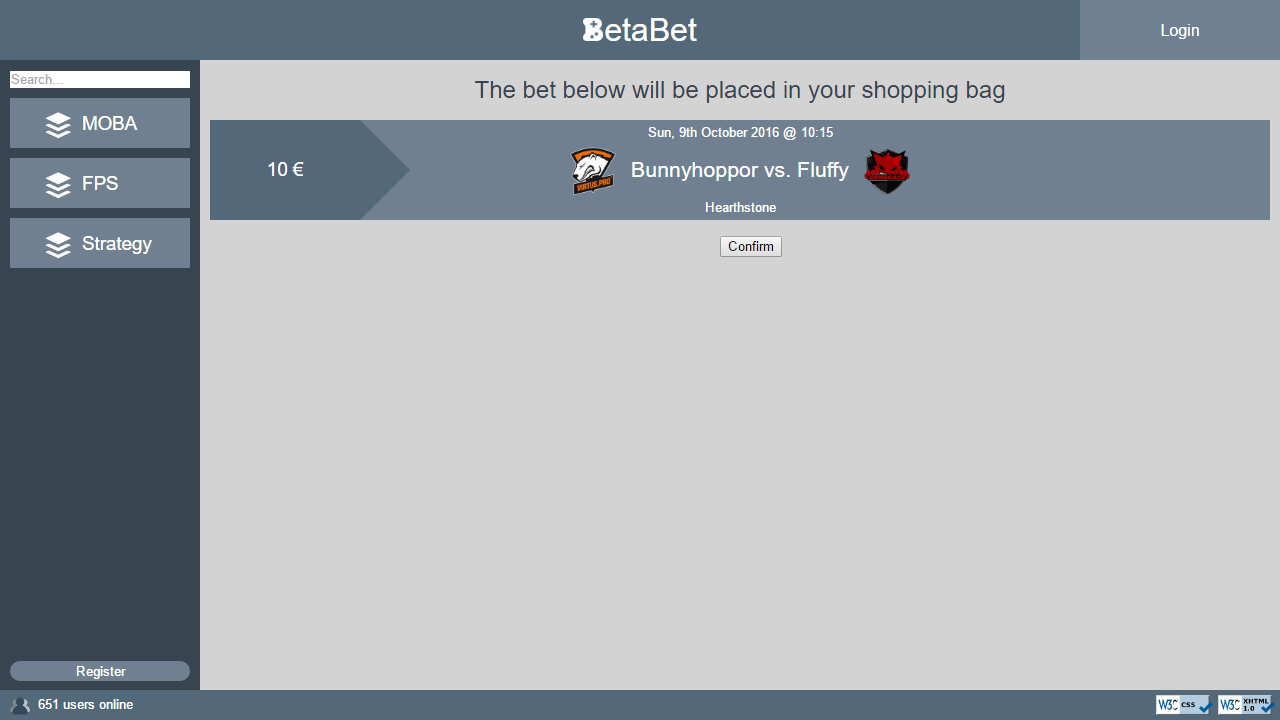
\includegraphics[width=\linewidth]{fig6}
    \caption{Confirmación de apuesta}
    \label{fig:fig6}
\end{minipage}
\smallskip\newline
Nota: Los botones \textit{Back} (\autoref{fig:fig5}) y \textit{Confirm} (\autoref{fig:fig6}) llevan al usuario de vuelta a la página principal.
\newpage
\subsection{Confirmar el carrito}
Si el carrito contiene una o más apuestas, aparece un botón en la esquina superior izquierda de la página indicando la cantidad total de dinero apostado. Al situar el puntero sobre este botón el texto cambia a \textit{Checkout}, y al pulsarlo se accede a la página de administración del carrito de apuestas.
\begin{center}
    \raisebox{-.5\height}{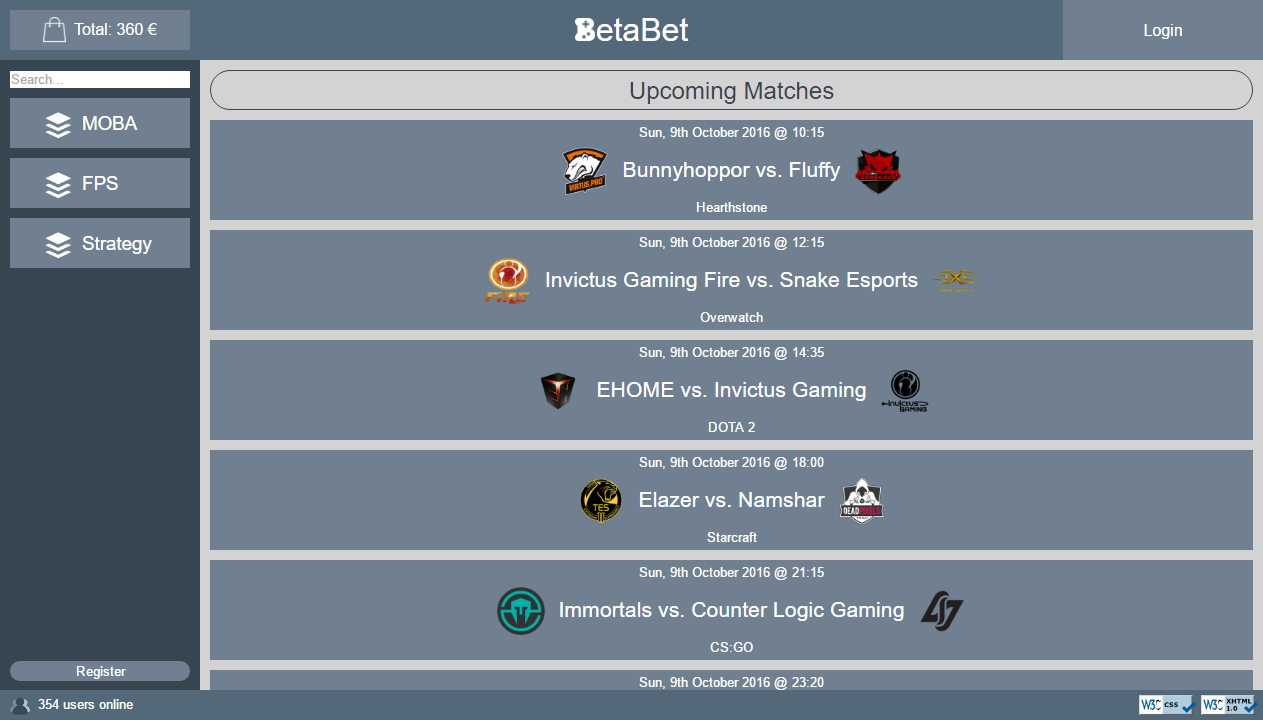
\includegraphics[width=.2\linewidth]{checkout1}}
    \raisebox{-.6\height}{\scalebox{2}{\myarrow}}
    \raisebox{-.5\height}{
\includegraphics[width=.2\linewidth]{checkout2}}
\end{center}
Esta página muestra todas las apuestas incluidas en el carrito junto con el dinero total que será apostado.
\smallskip\newline
\begin{minipage}{\linewidth}
    \centering
    \captionsetup{type=figure}
    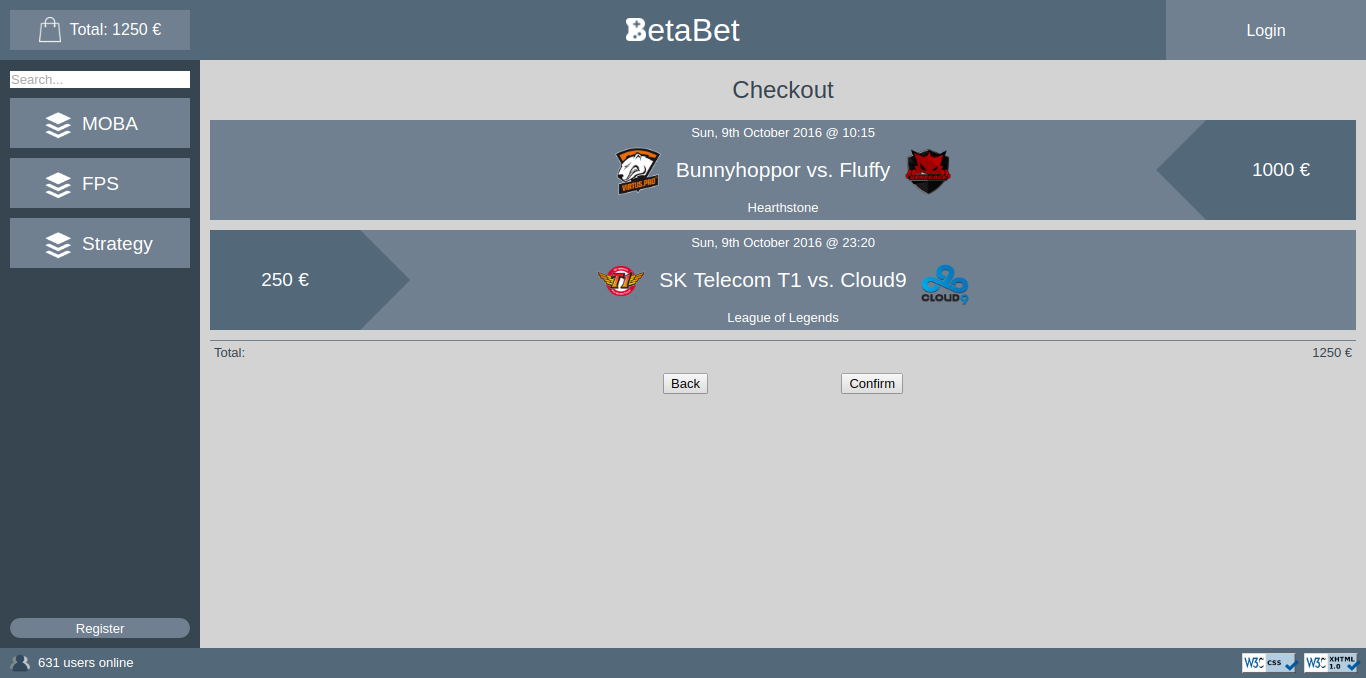
\includegraphics[width=\linewidth]{fig7}
    \caption{Carrito de apuestas}
    \label{fig:fig7}
\end{minipage}
\smallskip\newline
Situando el cursor sobre una apuesta del carrito, aparecen botones para modificar o eliminar dicha apuesta.
\begin{center}
    
\includegraphics[width=.8\linewidth]{checkout3}
\end{center}
La opción \textit{Edit} conduce al usuario a una página similar a \autoref{fig:fig5} que permite modificar apuesta inicial, mientras que \textit{Remove} muestra una confirmación equivalente a \autoref{fig:fig6} para eliminar la apuesta del carrito.
\smallskip\newline
Nota: Los botones \textit{Back} (\autoref{fig:fig5}) y \textit{Confirm} (\autoref{fig:fig6}) correspondientes en este caso vuelven a \textit{Checkout}.
\bigskip\newline
Una vez confirmado el carrito de apuestas, se comprueba que el usuario haya iniciado sesión y que tenga suficiente saldo en su cuenta. En caso contrario, se muestran los avisos pertinentes en el formulario.
\begin{multicols}{3}
    \begin{center}
        
\includegraphics[width=.975\linewidth]{checkout4}
        \cmark\,Confirmación exitosa del carrito
    \end{center}
    \columnbreak
    \begin{center}
        
\includegraphics[width=.975\linewidth]{checkout5}
        \xmark\,El usuario no ha iniciado sesión
    \end{center}
    \columnbreak
    \begin{center}
        
\includegraphics[width=.975\linewidth]{checkout6}
        \xmark\,Saldo insuficiente en la cuenta
    \end{center}
\end{multicols}
\subsection{Registrar un nuevo usuario}
\subsection{Iniciar sesión con un usuario}
\subsection{Consultar saldo de la cuenta}
\subsection{Ingresar o retirar saldo}
\subsection{Consultar el historial de apuestas}
\section{Implementación}
\section{Referencias}
\end{document}
